
%(BEGIN_QUESTION)
% Copyright 2012, Tony R. Kuphaldt, released under the Creative Commons Attribution License (v 1.0)
% This means you may do almost anything with this work of mine, so long as you give me proper credit

Use the ``impedance triangle'' to calculate the resistance ($R$) given the total impedance ($Z$) and the inductive reactance ($X$).  Also calculate the phase angle ($\theta$) of the total impedance:

$$\includegraphics[width=15.5cm]{i01937x01.eps}$$

\vskip 20pt

$R$ = 

\vskip 10pt

$\theta$ = 

\underbar{file i01937}
%(END_QUESTION)





%(BEGIN_ANSWER)

$R$ = 4.979 k$\Omega$

\vskip 10pt

$\theta$ = 16.77$^{o}$

%(END_ANSWER)





%(BEGIN_NOTES)

{\bf This question is intended for exams only and not worksheets!}.

%(END_NOTES)


